
%(BEGIN_QUESTION)
% Copyright 2007, Tony R. Kuphaldt, released under the Creative Commons Attribution License (v 1.0)
% This means you may do almost anything with this work of mine, so long as you give me proper credit

%A variety of chemicals are added to raw water when treating it for human consumption, and also when treating water for many industrial processes.  In the {\it coagulation} stage, chemicals are added to cause suspended solids in the raw water to coalesce into larger particles called {\it floc}, which precipitate out of solution more readily.  To maximize effectiveness and to reduce waste, these chemicals need to be added to the water in specific proportions:

Mange kjemikalier brukes for å behandle vann, før det blir drikkevann. I koaguleringssteget blir kjemikalier tilsatt for å få suspendert stoff til å koagulere til større partikler kalt fnokker. Fnokker er sedimentere eller lettere kunne filtreres. Disse kjemikaliene må blandes i et bestemt forhold. 

$$\includegraphics[width=15.5cm]{i01732x01.eps}$$

%If the raw water inlet flow and composition never change, the flocculant flow control setpoints may be left unchanged as well.  Once the correct proportions are set, the flocculant chemicals will continue to be added at just the right amounts.
Om innløpsvannet sin strømning eller sammensetning aldri forandrer seg. Kan settpunktet for tilsetting av kjemikalier v{\ae}re konstant. 

Men om strømningne på innløpsvannet varierer, må settpunktene varieres. Dette vil v{\ae}re tungvit og arbeidskrvende for operatøren, kan du komme opp med en løsning for forholdsregulering av dette systemet?

% But what if the raw water inlet flow {\it is} subject to change?  It would be quite inconvenient for operators to re-adjust the flocculant control setpoints every time a water flow rate change took place.  Can you think of a way to implement ratio control in this system to handle such changes automatically?

\vskip 20pt \vbox{\hrule \hbox{\strut \vrule{} {\bf Suggestions for Socratic discussion} \vrule} \hrule}

\begin{itemize}
\item{$\bullet$} For those who have studied flowmeter technology, identify the types of flowmeters shown in this diagram and explain how each of them works.
\item{$\bullet$} After implementing your control strategy, analyze the effects of the raw water flow transmitter failing with a {\it low} signal.
\medskip

\underbar{file i01732}
%(END_QUESTION)





%(BEGIN_ANSWER)

I'll let you sketch a possible solution to this problem!

\vskip 10pt

Follow-up question: identify each flowmeter type, and explain their respective operating principles!

%(END_ANSWER)





%(BEGIN_NOTES)

Here is one possibility:

$$\includegraphics[width=15.5cm]{i01732x02.eps}$$

Polymer-based flocculants often have the undesirable effect of lowering the water's pH, which is not only bad for drinking purposes, but also bad because effective flocculation cannot occur if the pH is too low.  Lime powder is often added to the water in order to offset the low pH of the flocculant.  This lime flow may also be controlled by flow ratio, trimmed by a pH sensor and pH controller.

%INDEX% Control, strategies: ratio
%INDEX% Process: municipal water flocculation

%(END_NOTES)


